\subsection{fast convolution}

\begin{frame}{fast convolution}{introduction}
	convolution: measure impulse response h(i) and apply FIR filter to signal
	\begin{eqnarray}
		y(i) &=& x(i) \ast h(i)\\
			 &=& \sum\limits_{j=-\infty}^{\infty}{h(j)\cdot x(i-j)}\\
		Y(z) &=& X(z) \cdot H(z)
	\end{eqnarray}
\end{frame}

\begin{frame}{DFT convolution}{signal and impulse response 1/2}
	\begin{itemize}
		\item	multiplication: length of $H(z) = M$ must equal length of $X(z) = N$
		\item	minimum DFT length: $L \leq M+N-1$
	\end{itemize}
	\only<1>{
	\begin{figure}
		\centering
			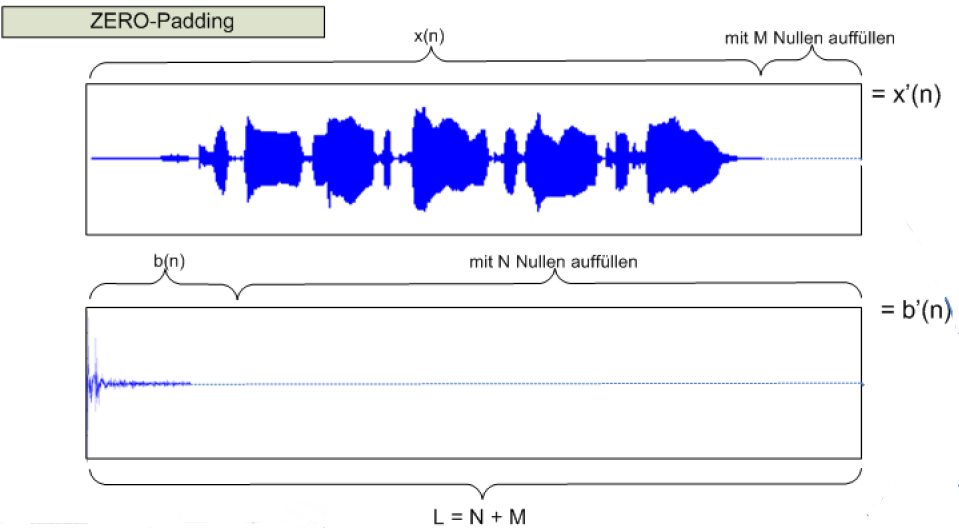
\includegraphics[scale=.4]{graph/conv_dft_zp}
	\end{figure}
	}
	\only<2->{
	\begin{enumerate}
		\item	$X = DFT(x'(i))$
		\item	$H = DFT(h'(i))$
		\item	$Y = X\cdot H$
		\item	$y = DFT^{-1}(Y)$
        \item   throw away zeros if DFT was longer than $M+N$
	\end{enumerate}
	}
	\only<3>{
	\begin{figure}
		\centering
			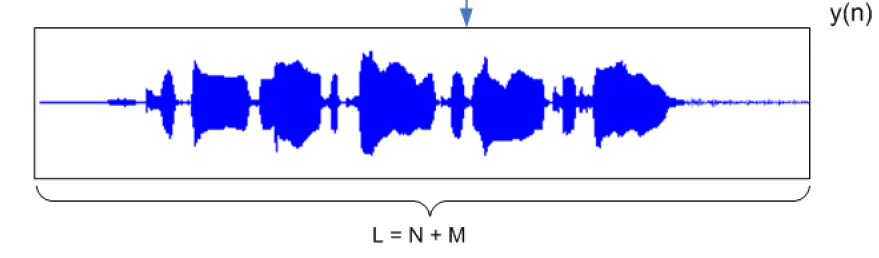
\includegraphics[scale=.4]{graph/conv_dft_res}
	\end{figure}
	}
	\vspace{50mm}
\end{frame}

\begin{frame}{DFT convolution}{signal and impulse response 2/2}
	\textbf{properties}:
	\begin{itemize}
		\item	no real-time: signal has to be known completely
		\item	high memory requirements (signal length $N$ + impulse response length $M$)
		\begin{itemize}
            \item	when FFT: next larger power of two
        \end{itemize}
	\end{itemize}
\end{frame}

\begin{frame}{FFT convolution}{blocked signal and impulse response 1/2}
	\begin{enumerate}
		\item	split input signal into blocks of length $M$
		\item	DFT convolution with each block (zeropadding)
		\item	overlap and save
	\end{enumerate}
	\only<1>{
	\begin{figure}
		\centering
			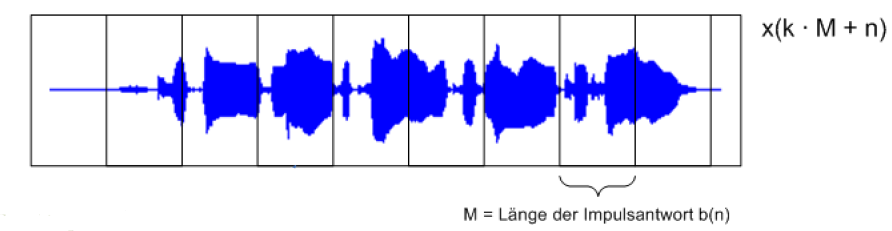
\includegraphics[scale=.4]{graph/conv_dft_split}
	\end{figure}
	}
	\only<2>{
	\begin{figure}
		\centering
			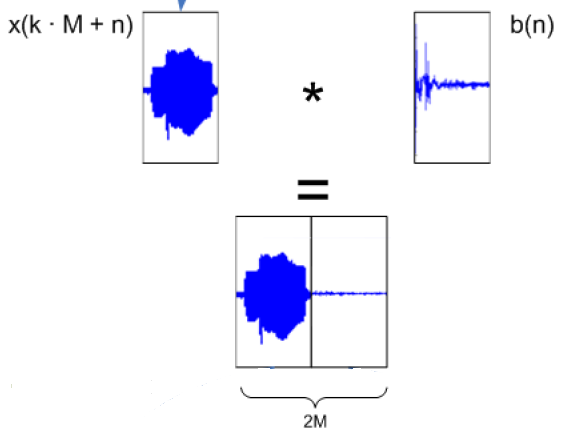
\includegraphics[scale=.4]{graph/conv_block}
	\end{figure}
	}
	\only<3>{
	\begin{figure}
		\centering
			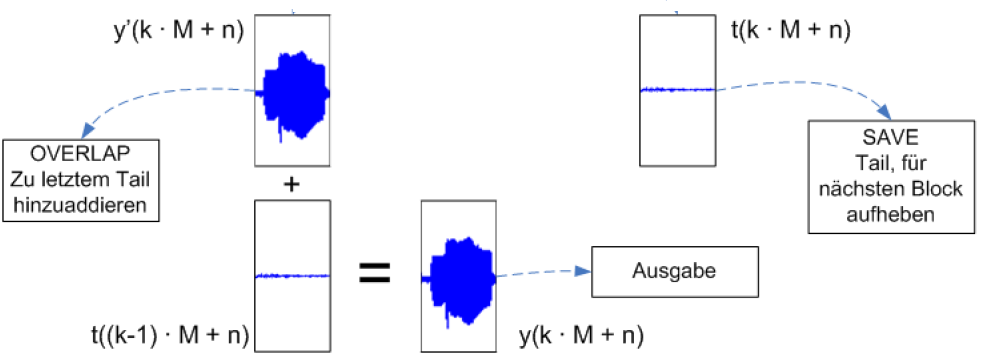
\includegraphics[scale=.4]{graph/conv_overlapsave}
	\end{figure}
	}
	\only<4>{
	\begin{figure}
		\centering
			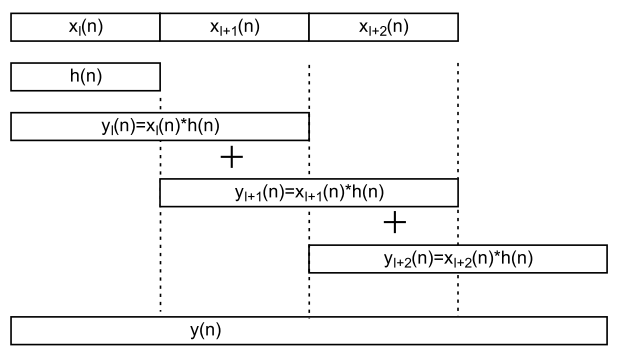
\includegraphics[scale=.5]{graph/conv_block2}
	\end{figure}
	}
	\vspace{50mm}
\end{frame}

\begin{frame}{FFT convolution}{blocked signal and impulse response 2/2}
	\textbf{properties}:
	\begin{itemize}
		\item	minimum latency: impulse response length
		\item	long FFT, but more efficient
		\item	FFT of impulse response \textit{is only computed once}
	\end{itemize}
\end{frame}

\begin{frame}{partitioned convolution}{blocked signal and blocked impulse response 1/3}
	\begin{enumerate}
		\item	split \textbf{both} input signal and impulse response into blocks of arbitrary length
		\item	DFT convolution with each signal block with each impulse response block (zeropadding)
		\item	overlap and save
	\end{enumerate}
	\only<1>{
	\begin{figure}
		\centering
			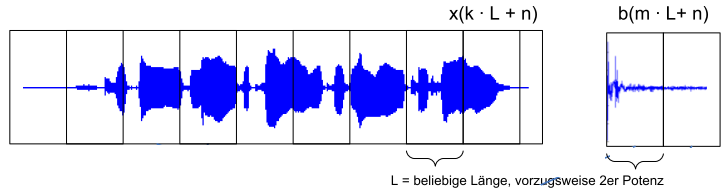
\includegraphics[scale=.4]{graph/conv_blockblock}
	\end{figure}
	}
	\only<2>{
	\begin{figure}
		\centering
			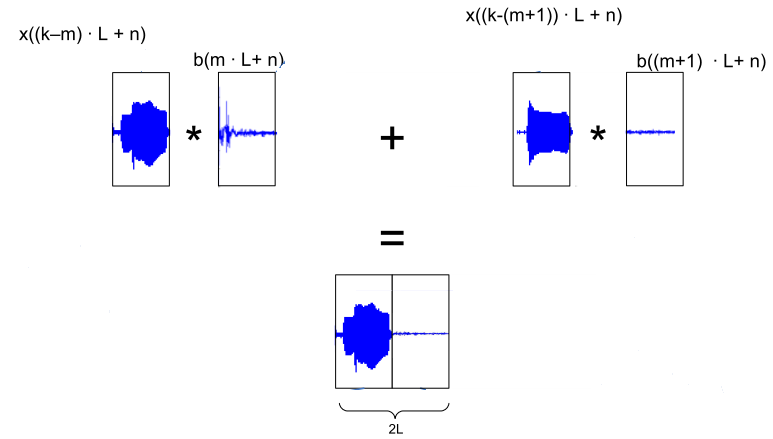
\includegraphics[scale=.4]{graph/conv_fast}
	\end{figure}
	}
	\only<3>{
	\begin{figure}
		\centering
			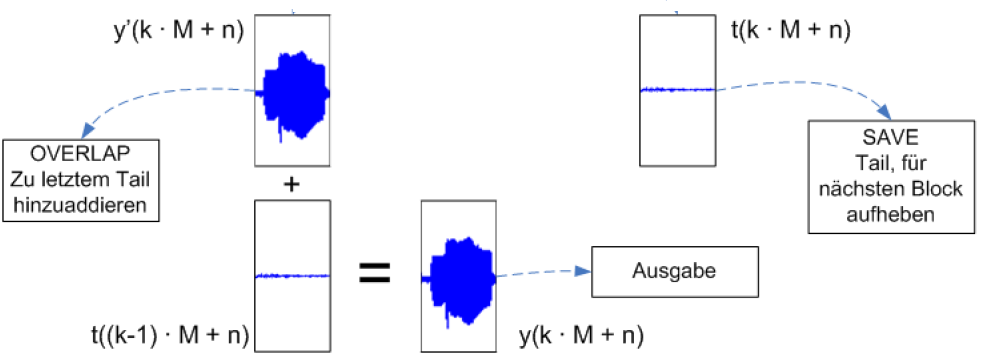
\includegraphics[scale=.4]{graph/conv_overlapsave}
	\end{figure}
	}
	\vspace{50mm}
\end{frame}

\begin{frame}{partitioned convolution}{blocked signal and blocked impulse response 2/3}
	\vspace{-5mm}
    \begin{figure}
		\centering
			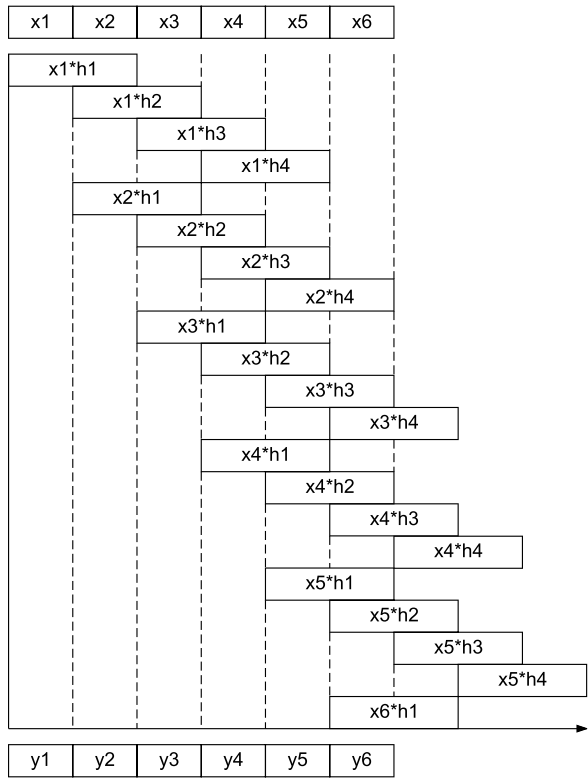
\includegraphics[scale=.35]{graph/conv_fast2}
	\end{figure}
\end{frame}

\begin{frame}{partitioned convolution}{blocked signal and blocked impulse response 3/3}
	\textbf{properties}:
	\begin{itemize}
		\item	arbitrary choice of latency/FFT length 
			\begin{itemize}
				\item	long FFT: high latency, low workload
				\item	short FFT: short latency, high workload
			\end{itemize}
		\item	FFTs of IR computed only once
	\end{itemize}
\end{frame}

\begin{frame}{non-uniform partitioned convolution}{different block lengths}
	\begin{itemize}
		\item	fast convolution: latency still formidable for efficient implementation
		\pause
		\item[$\Rightarrow$] \textbf{non-uniform block lengths}
	\end{itemize}
		\begin{figure}
		\centering
			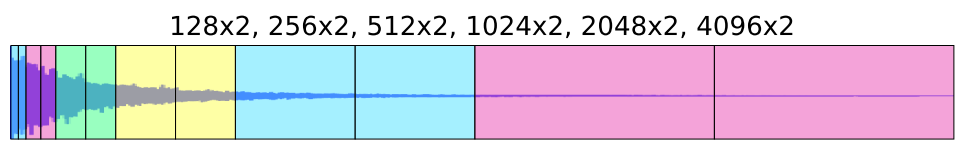
\includegraphics[scale=.4]{graph/conv_nonuniform}
	\end{figure}
    \pause
    \begin{itemize}
        \item   \textbf{advantages}:
            \begin{itemize}
                \item   \textit{any} desirable latency
            \end{itemize}
        \item   \textbf{disadvantages}:
            \begin{itemize}
                \item   less efficient due to multiple FFT lengths (but: inefficiency of short FFT partly compensated by very long FFTs)
                \item   complex implementation
                \item   comparably high memory usage (IR in many different FFT lengths)
            \end{itemize}
    \end{itemize}

\end{frame}

